% 1977 年四川卷参考题一(3)：抛物线 y=x^2 与 x=y^2 所围区域 (D)（浅灰填充）
% 交点 (0,0) 与 (1,1)，右侧标注 y=x^2、x=y^2、(1,1)，区域内标 D（按源卷第 7 页布局）
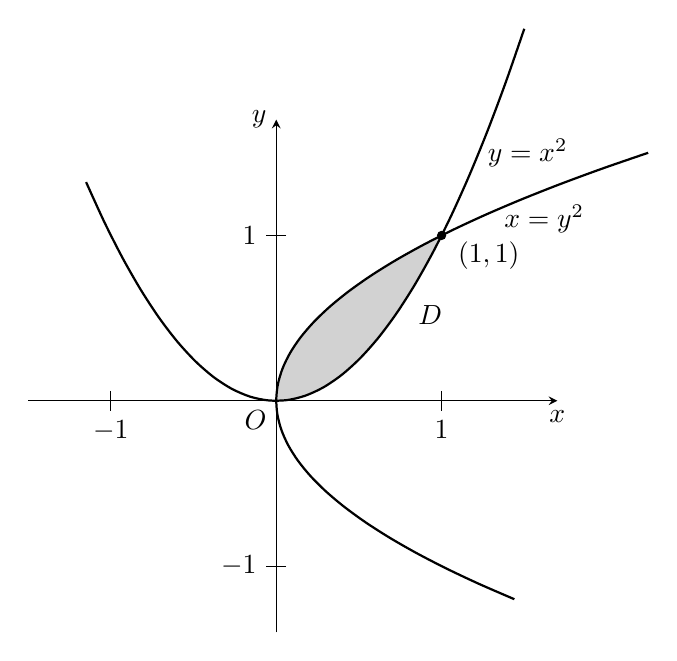
\begin{tikzpicture}[scale=2.1,>=stealth]
  \draw[->] (-1.5,0)--(1.7,0) node[below] {$x$};
  \draw[->] (0,-1.4)--(0,1.7) node[left] {$y$};
  \node[below left] at (0,0) {$O$};
  % 区域 (D)：0≤x≤1 上 y=x²（下）与 y=√x（上）之间
  \fill[gray!35]
    (0,0) plot[domain=0:1,smooth] (\x,{\x*\x})
    -- plot[domain=1:0,smooth] (\x,{sqrt(\x)}) -- cycle;
  \draw[thick,domain=-1.15:1.5,smooth] plot (\x,{\x*\x});
  \draw[thick,domain=-1.2:1.5,smooth,samples=30] plot ({\x*\x},{\x});
  \fill (1,1) circle (0.8pt);
  \node[right] at (1.04,0.88) {$(1,1)$};
  \node[right] at (0.80,0.52) {$D$};
  \node[right] at (1.22,1.50) {$y=x^2$};
  \node[right] at (1.32,1.10) {$x=y^2$};
  \foreach \x in {-1,1}{
    \draw[thin] (\x,0.06)--(\x,-0.06) node[below] {$\x$};
  }
  \foreach \y in {-1,1}{
    \draw[thin] (0.06,\y)--(-0.06,\y) node[left] {$\y$};
  }
\end{tikzpicture}
